This section describes Ascent's primary abstractions and surveys its general capabilities.
%
Ascent organizes its capabilities into five types of in situ tasks, which
it refers to as \textbf{actions}.
%
Its five actions are:
\begin{itemize}
\item \textbf{Pipelines} transform data from one form to another.
%
\item \textbf{Scenes} render images.
%
\item \textbf{Extracts} are used to move data out of Ascent, i.e., to file I/O or to another framework.
%
\item \textbf{Queries} provide quantitative summarizations of the data.
%
\item \textbf{Triggers} adapt when other actions are executed, based on the conditions of the simulation.
%
\end{itemize}

These actions are highly interoperable, and Ascent can employ multiple actions of the same type
at once.
%
Consider the following example of Ascent doing in situ analysis on an input data set, $D$,
for a given cycle of a simulation.
%
Ascent begins by applying an isosurfacing operation to $D$ to make a new data set $D'$ (pipeline).
%
It then applies a trigger to $D'$ --- it takes the surface area of the isosurface (query) and compares
the total area with the area from the previous time it was executed.
%
If the total area has changed by more than 5\%, then Ascent would render an image of $D'$ (scene)
and also save the original data set $D$ to disk (extract).
%
Going beyond this example, it is possible to have multiple triggers, arbitrary conditions for
the triggers (queries or otherwise), as well as many pipelines, scenes, and extracts.
%
Fig.~\ref{fig:ascent_example} shows an example of this, specifically two pipelines and two extracts.

\begin{figure}
\centering
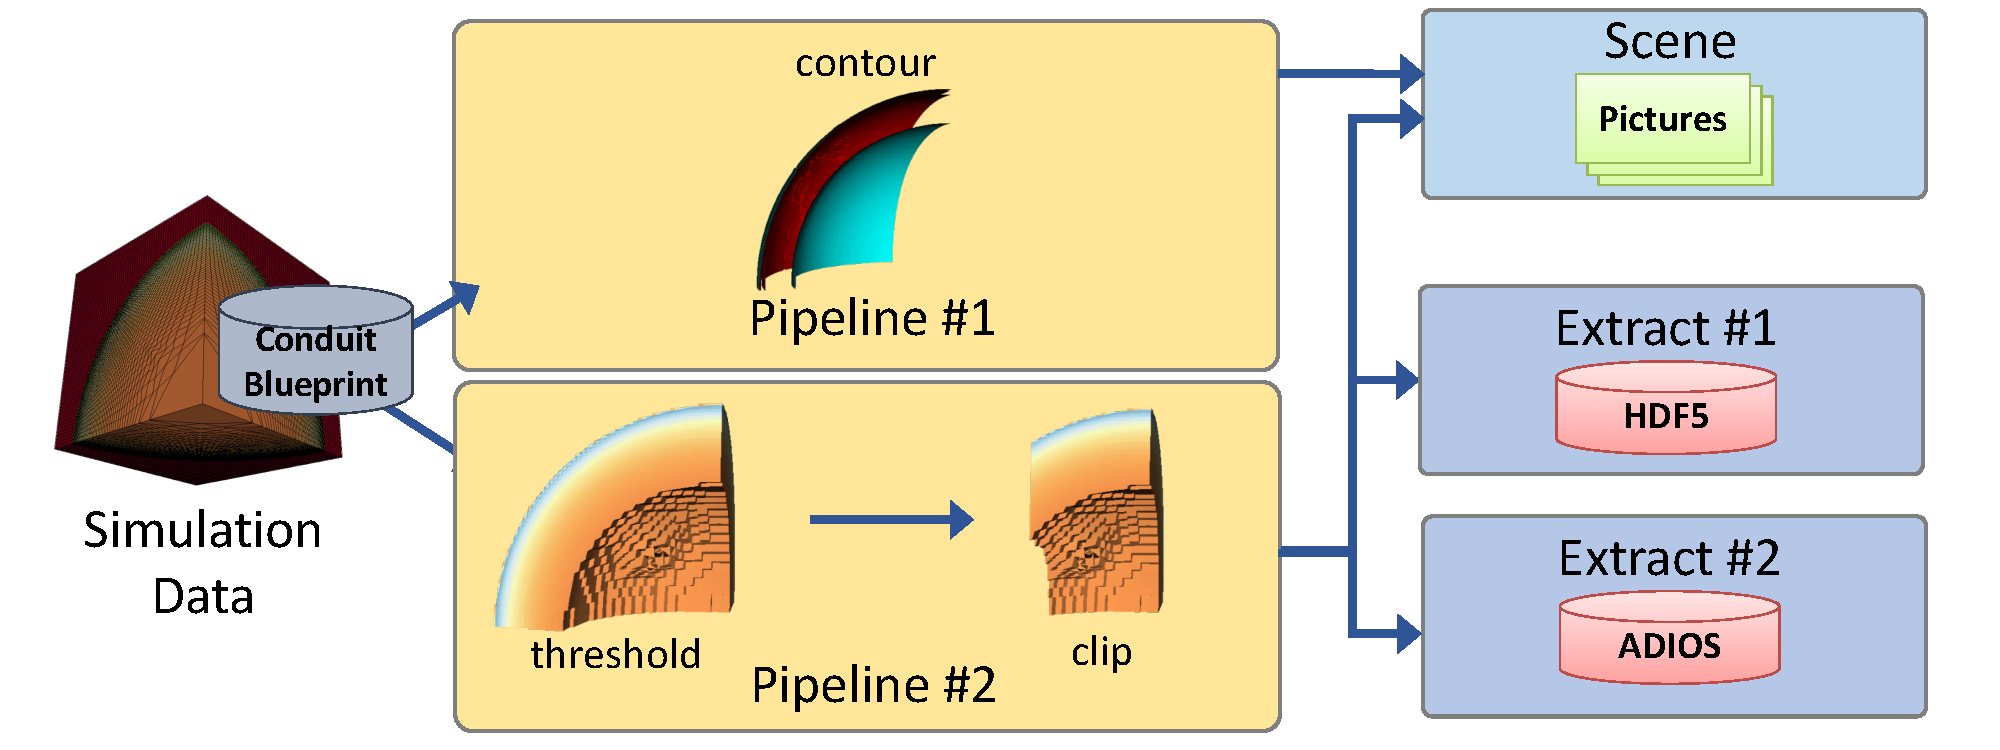
\includegraphics[width=\textwidth]{images/ascent_actions_diagram.pdf}
\caption{\label{fig:ascent_example} An example of how Ascent actions can be combined.
In this example, simulation data is acquired from Conduit/Blueprint (see \S\ref{sec:API}),
and that data is relayed into two pipelines (labeled \#1 and \#2).
The first pipeline applies a contour operation, while the second
applies threshold and clip operations.
%
The results of these pipelines are used in multiple ways.
A scene uses both pipelines as input, while two extracts use only the second pipeline
as input, outputting using two different I/O libraries.}
\end{figure}

\subsection{Pipelines}

Pipelines allows users to describe a series of data transformations, also known as filters,
to execute on simulation data.
%
%These data transformations are sometimes referred to as filters in other
%frameworks (like VTK~\cite{VTK}), and
Fig.~\ref{fig:ascent_example} shows
typical filters for visualization: contour, threshold, and clip.
%Figure~\ref{img:pipelines} shows two examples of pipelines.
%%
%Pipeline \#1 creates contours from a simulation field, and pipeline \#2
%thresholds cells that are within a scalar range then applies a clipping operation.
%
Ascent allows users can define an arbitrary number of pipelines.
%
In terms of inputs and outputs, the input to a pipeline is either
the simulation data or another pipeline, and the outputs of a pipeline
can go to scenes, extracts, and queries.
%
Further, triggers can make use of pipelines, and their relationship is discussed further
in \S\ref{sec:ascent:triggers}.

%
%The default source of pipelines, and all other actions, is the data
%published by the simulation, but all actions can consume the results
%of declared pipelines, including other pipelines.

%\begin{figure}
%\centering
%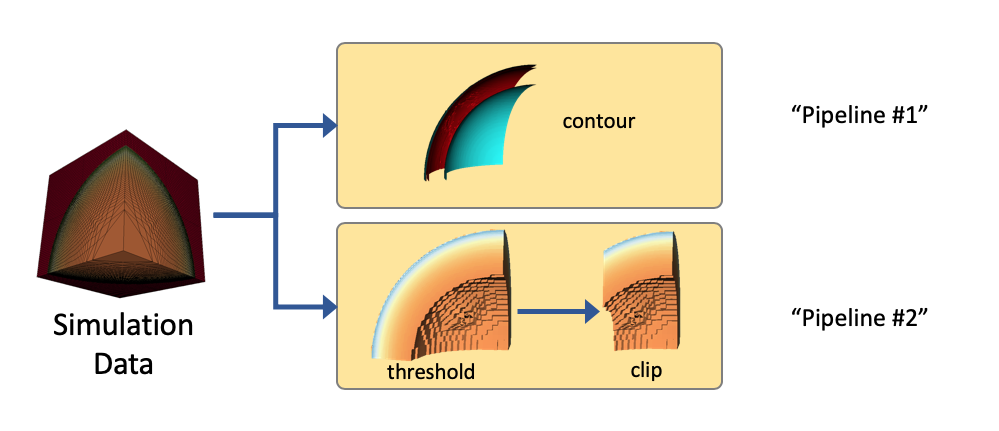
\includegraphics[width=0.6\textwidth]{images/pipelines}
%\caption{\label{img:pipelines} Examples pipelines that transforms simulation data via visualization operators.}
%\end{figure}

Notable filters currently supported by Ascent include:
\begin{multicols}{2}
\begin{itemize}
\item Clipping
\item Contour
\item Histogram
\item Isovolume
\item Particle Advection
\item Statistics
\item Slice
\item Threshold
\end{itemize}
\end{multicols}

There are also filters that create new fields: Divergence, Gradient, Logarithm, Q-Criterion, Vector Magnitude, and Vorticity.
%
Finally, Ascent contains two \fix{in situ-specific} filters --- Lagrangian Flow
and Sampling (\fix{should be a reference here to Biswas chapter on sampling})
--- that
reduce data size significantly enough that it can be saved to disk and explored post hoc.



\subsection{Scenes}

Scenes create images.
%
They typically operate on the output of pipelines, but they also can work directly
on the original simulation data.
%
Scenes do not return anything to Ascent that can interact with other actions, but they
do save the images they produce to disk for later inspection.

A scene is made up of ``renders" and ``plots".
%
Renders can be thought of as sub-scenes, i.e., each scene is made up of many sub-scenes (renders),
which contain
camera specifications, image dimensions, background and
foreground colors, and annotation controls.
%
There can be an arbitrary number of renders for a scene. 
%
Plots are the things to render.
%
A plot consists of two things: what data to render and how to render it.
%
The data comes from the input (usually a pipeline), and the method for rendering the data can vary.
%
Currently, Ascent supports four plot types: pseudocolor, mesh, volume
rendering, and radiograph plots (see Fig.~\ref{fig:ascent_plots}).
%
Each of these plot types contain parameters that control the input data
(name of the pipeline to consume, which scalar field to operate on, etc.)
and how to carry out the rendering (color tables, scalar ranges, etc.).
%

\begin{figure}
\centering
  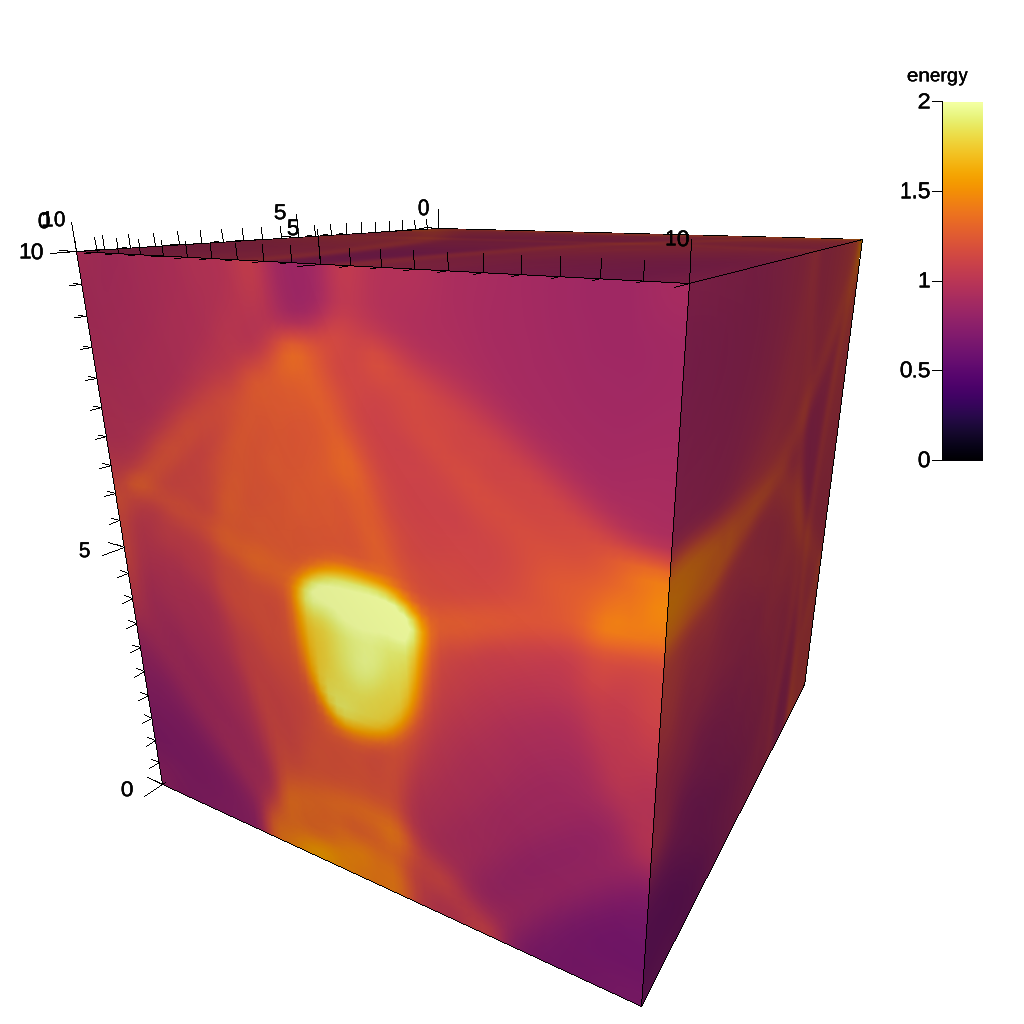
\includegraphics[width=0.4\textwidth]{images/pseudocolor250}
  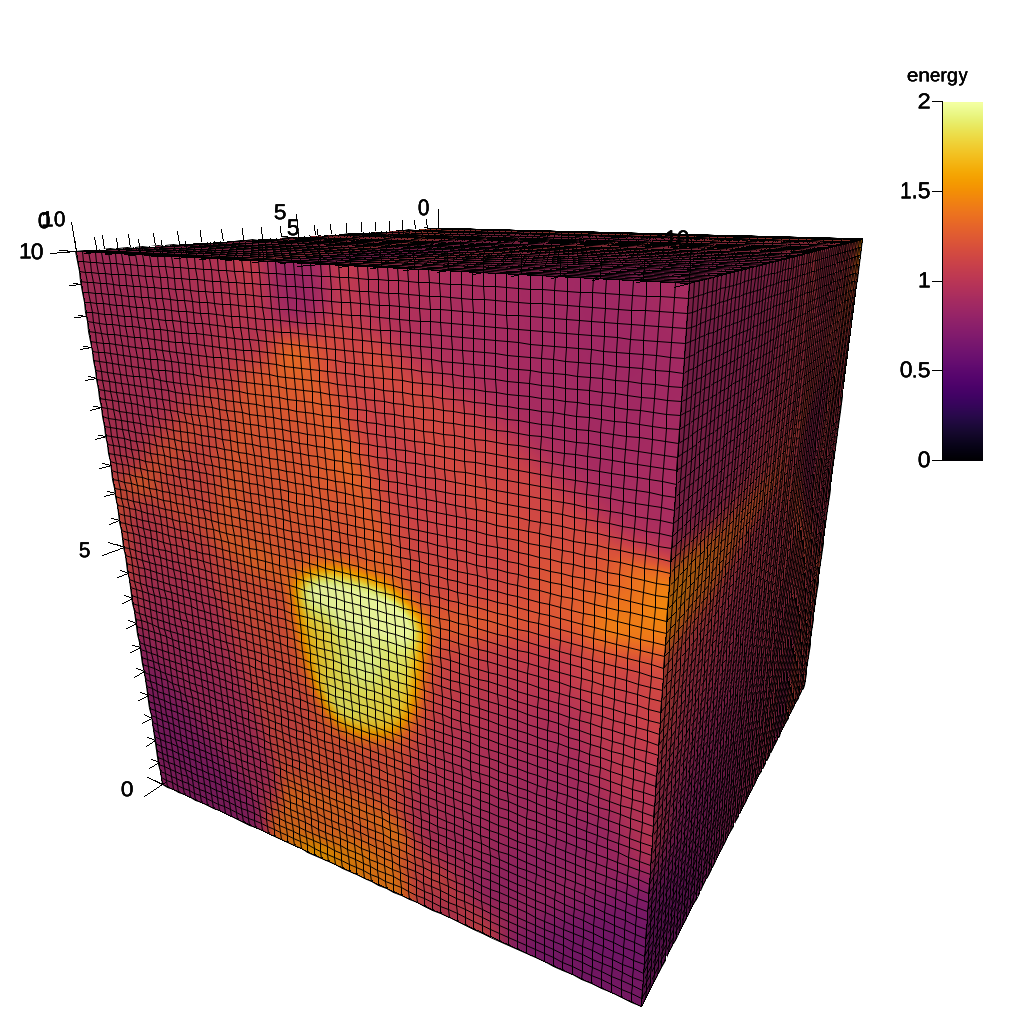
\includegraphics[width=0.4\textwidth]{images/mesh250}
  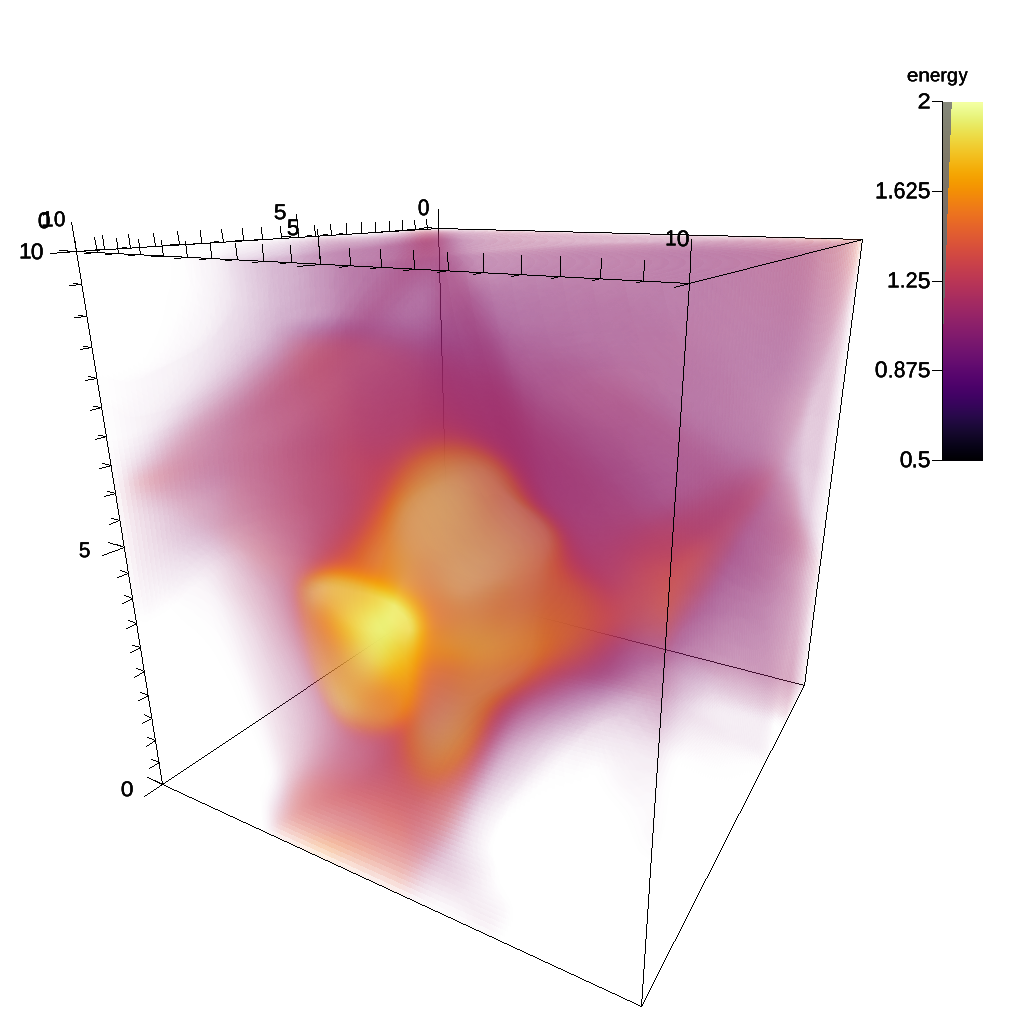
\includegraphics[width=0.4\textwidth]{images/volume250}
  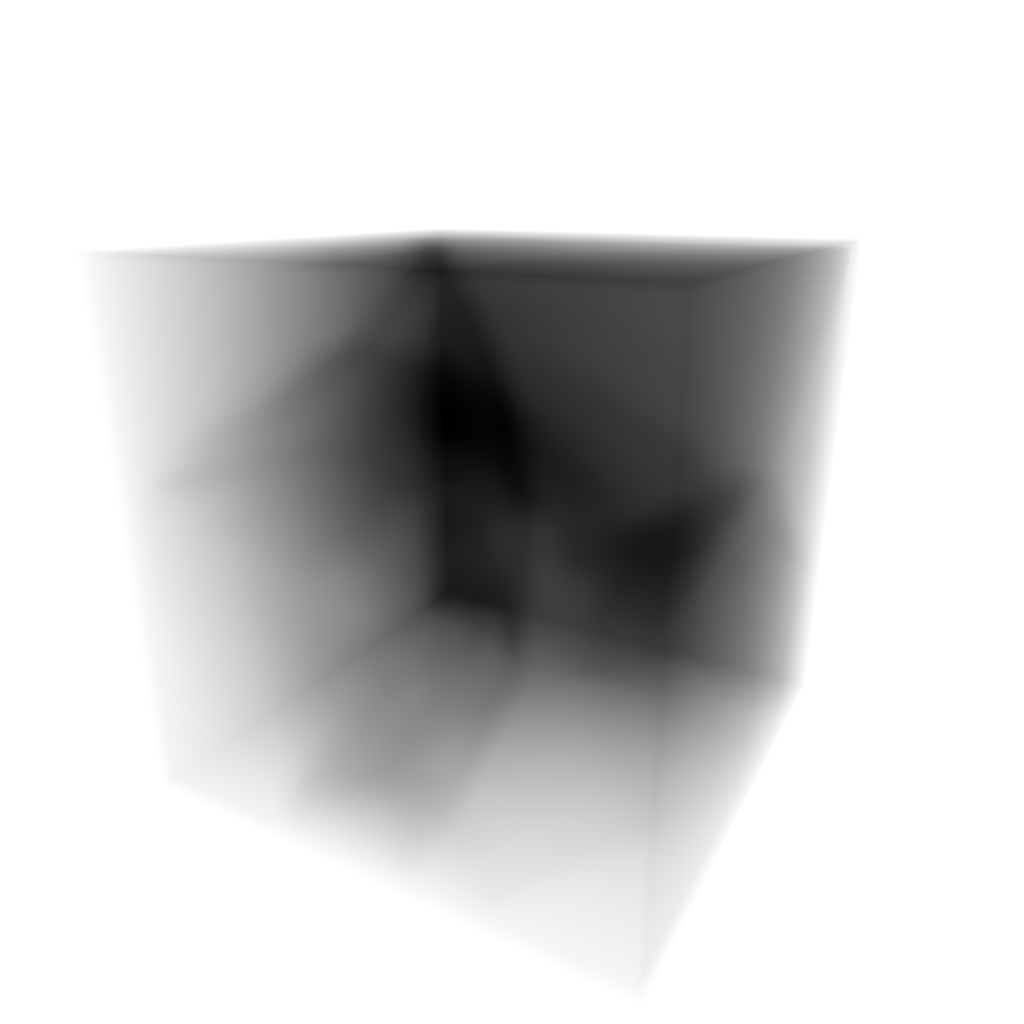
\includegraphics[width=0.4\textwidth]{images/radiograph250}
  \caption{\label{fig:ascent_plots} Example images of Ascent's four plot types:
pseudocolor (top left), mesh (top right, which also includes a pseudocolor plot),
volume rendering (bottom left), and radiograph (bottom right).
%
The data for these images comes from CloverLeaf3D, 
a hydrodynamics proxy-application included with Ascent.
  }
\end{figure}

In terms of camera placement,
Ascent creates a default camera based on the bounding box of the data set 
that faces the data set.
%
Renders inherit the default camera parameters, simplifying creation of useful
cameras positions.
%
Ascent also provides simple controls to rotate the camera on the
sphere circumscribing the data set.
%
Of course, the user is free to set all
camera parameters explicitly as well.

Finally, scenes can create Cinema~\cite{AhrensCinema} databases, i.e.,
a large set of images that can be explored after the simulation.
\fix{Should be a reference to Cinema chapter here.}

%Currently supported plots include:
%\begin{itemize}
%\item Pseudocolor
%\item Mesh
%\item Volume
%\item Radiograph
%\end{itemize}

\subsection{Extracts}
The extracts action covers a broad range of activities.
%
The common theme among these activities is moving data outside Ascent.
%
The word extract is meant to convey ``extracting'' data from Ascent to somewhere else.
%
%
%Extracts are an escape hatch in Ascent that enables data to be sent
%outside of Ascent.
%
Extracts can be as simple as saving data to HDF5 files.
%
That said, extracts are also the mechanism to integrate other tools with Ascent --- a gateway
to a larger workflow.
%
This is important because
Ascent does not have the long tail of functionality that tools like ParaView or VisIt provide, which
were built over decades of development.
%
Through extracts, Ascent can pass data directly to ParaView Catalyst~\cite{Catalyst}.
%
Another example of using extracts to provide additional functionality is the
ADIOS~\cite{Lofstead2008} extract, which allows Ascent to link to in transit workflows.

Ascent supports connections to the Python ecosystem through its Python and
Jupyter extracts~\cite{CyrusISAV,Jupyter}.
%
Python extracts execute custom analysis code provided by the user, and the
Jupyter extracts allow for incoming Jupyter notebooks connections from a web
browser.

We feel that the Jupyter notebook interface is an important future direction
for Ascent, and for in situ as a whole.
%
One of in situ's greatest weaknesses is the reliance on a priori
knowledge, and one strategy to mitigate this weakness is incorporating a human-in-the-loop.
%
Through the Jupyter notebook interface, users can pause a running simulation
and interact with the data.
%
Additionally, Jupyter widgets enable fast prototyping of domain specific GUIs.

\fix{Do these new cites?} In all, currently supported extracts include:
\begin{itemize}
\item ADIOS
\item Babel Flow~\cite{babelflow}
\item Jupyter Notebooks
\item ParaView Catalyst
\item Python
\end{itemize}

\subsection{Queries}
\label{action_queries}
Queries enable users to ask quantitative questions.
%
The inputs to a query can take a varied form:
the simulation data directly,
the data produced by a pipeline,
or even a combination of multiple pipelines and simulation data.
%
That said, typical queries are used to access the current state of the simulation
and to summarize data.
%
The results of queries are saved in Ascent's state.
%
These results can then be used to
interact with other actions --- a query's return value can be turned
into the parameter for another action (for example setting the camera position in a scene based
on the result of a bounding box query) or it can be used to affect triggers.
%

The mechanism behind queries enables powerful operations.
%
Queries are formed via a Python-like language that
enables expressions for math operations,
call functions, and evaluating conditionals.
%
Further, since the results of queries are stored into named identifiers, subsequent queries
can build on the results of other queries, allowing for complex combinations.
%
%Examples include min-max queries, statistics, cell locations,
%and probability distributions.
%
This also enables creating a ``time history,'' since
Ascent can call the same query every time step and accumulate the result.

%Queries are executed each time Ascent is called, and the resulting time
%history can be saved, accessed by the simulation, or accessed in other
%expressions.

%Queries can be as simple as calling a function that returns the current simulation cycle
%and storing it into a variable.
%
%More complex queries can calculate the amount of entropy of a field.
%

Examples of queries include:
\begin{itemize}
\item $cycle()$: calling a function that returns the current simulation cycle and storing it into a variable.
\item $max(field('pressure'))$: the maximum value of the pressure field.
\item $entropy(histogram(field('gyre'), num\_bins=128))$: calculating a histogram of the gyre field with 128 bins, and then calculating the entropy of that histogram.
\end{itemize}
%Listing~\ref{simple_query} shows the declaration of a query that returns
%the current simulation cycle and stores it into a variable identifier \textit{cycle},
%and Listing~\ref{complex_query} shows a more complex example of a query that
%calculates the entropy of a simulation field.
%\begin{lstlisting}[language=Python,caption={Examples of querying the simulation cycle}, label={simple_query}]
%# add a simple query expression (q1)
%queries["q1/params/expression"] = "cycle()"
%queries["q1/params/name"] = "cycle"
%\end{lstlisting}
%

%
%
%\begin{lstlisting}[language=Python,caption={A more complex example of queries in Ascent}, label={complex_query}]
%# add a more complex query expression (q2)
%queries["q2/params/expression"] = "entropy(histogram(field('gyre'), num_bins=128))"
%queries["q2/params/name"] = "entropy_of_gyre"
%\end{lstlisting}

\subsection{Triggers}
\label{sec:ascent:triggers}

Triggers are designed to balance the tensions between cost and capturing important phenomena.
%
In a typical scenario, in situ visualization is performed at regular intervals, e.g.,
every $X$ simulation cycles or every $M$ minutes of wall clock time.
%
This approach creates a tension between two important goals:
(1) achieving the visualizations and analyses at the right times within the simulation
and (2) minimizing costs.
%
On the one hand, performing visualization frequently maximizes the chances of having
visualizations at the right times (and likely also some uninteresting times), but
is costly,  e.g., adding a 50\% overhead on top of the simulation.
%
On the other hand, performing visualization infrequently minimizes costs, but also makes it
less likely that the visualizations will occur during important phenomena.
%

Triggers operate in two phases: inspection and action/inaction.
%
The purpose of the inspection phase is to determine if the action should be taken.
%
The trigger should ``fire'' if the action should be taken.
%
Further, if the inspection routine is cheap (i.e., executes quickly) and accurate (i.e.,
fires at the right times), then
triggers can be an effective strategy.
%
In this case, triggers can be called frequently (possibly every cycle) and still minimize cost
(since the visualization in the action/inaction phase is called only when necessary) and
get the right information (since the trigger is accurate).
%
Of course, triggers make the most sense when the desired visualization is quite expensive
to calculate;
if the desired visualization could be calculated as quickly as the inspection,
then there is no cost benefit.





%Traditional in situ actions execute every $X$ simulation cycles, this presents
%two related problems.
%
%First, if the analysis is expensive, then the total cost of the action may exceed
%what a user is willing to pay,
%
%Second, if the analysis called infrequently, then the feature or event that the analysis is
%trying to capture could easily be missed.
%
%Triggers address these issues by coupling inspection routines with analysis, and a
%potentially costly analysis only executes when user defined precondition is met.
%
%Ideally, inspection routines are cheap and can be called every cycle, while the analysis
%that are ``triggered'' can cost more.

A trigger is made up of two parts; for clarity, we term these two parts 
as trigger-condition and trigger-action.
(A trigger-action is only executed if the trigger-condition is true.)
%
In Ascent, any conditional expression can be a trigger-condition, although most trigger-conditions
incorporate the queries and expressions infrastructure from
\S\ref{action_queries}.
%
Trigger-actions utilize Ascent's other actions: pipelines, extracts, scenes, and
queries.  
%
For example, a trigger-action may be to calculate an isosurface (pipeline) and save
an image (scene).
%The part for the action incorporates 
%When the condition evaluates to true, the trigger fires, executing a user provided
%set of actions, which can be any Ascent action.
%
In practice, triggers are often used for debugging (e.g., saving data to
a file when invalid values are found) or 
for capturing information when a phenomena occurs
(e.g., saving an image when the maximum value of a field exceeds a threshold from the
previous value).
%
%When an event can be expressed in these terms, triggers are a powerful tool for
%maximizing constrained resources in situ.

Examples of trigger-conditions in Ascent include:
\begin{itemize}
\item $cycle() > 100 \ and \ cycle() < 200$: the cycle field is
between 100 and 200.
\item $max(field('pressure')) > 100.0$: the max value of the pressure field
exceeds 100.
\item $magnitude(max(field('braid')).position - vector(0,0,0)) > 0$\fix{: ??}
\end{itemize}

\subsection{Interactions Between Actions}

Although some of the interactions between Ascent actions have been mentioned previously,
this subsection formalizes and summarizes these interactions.
%
The key takeaway is that \fix{pathing?} between actions in Ascent is important and well-supported.
%
This is not always the case; in some projects, interoperability between different types of actions
can be difficult or impossible.

\begin{figure}
\centering
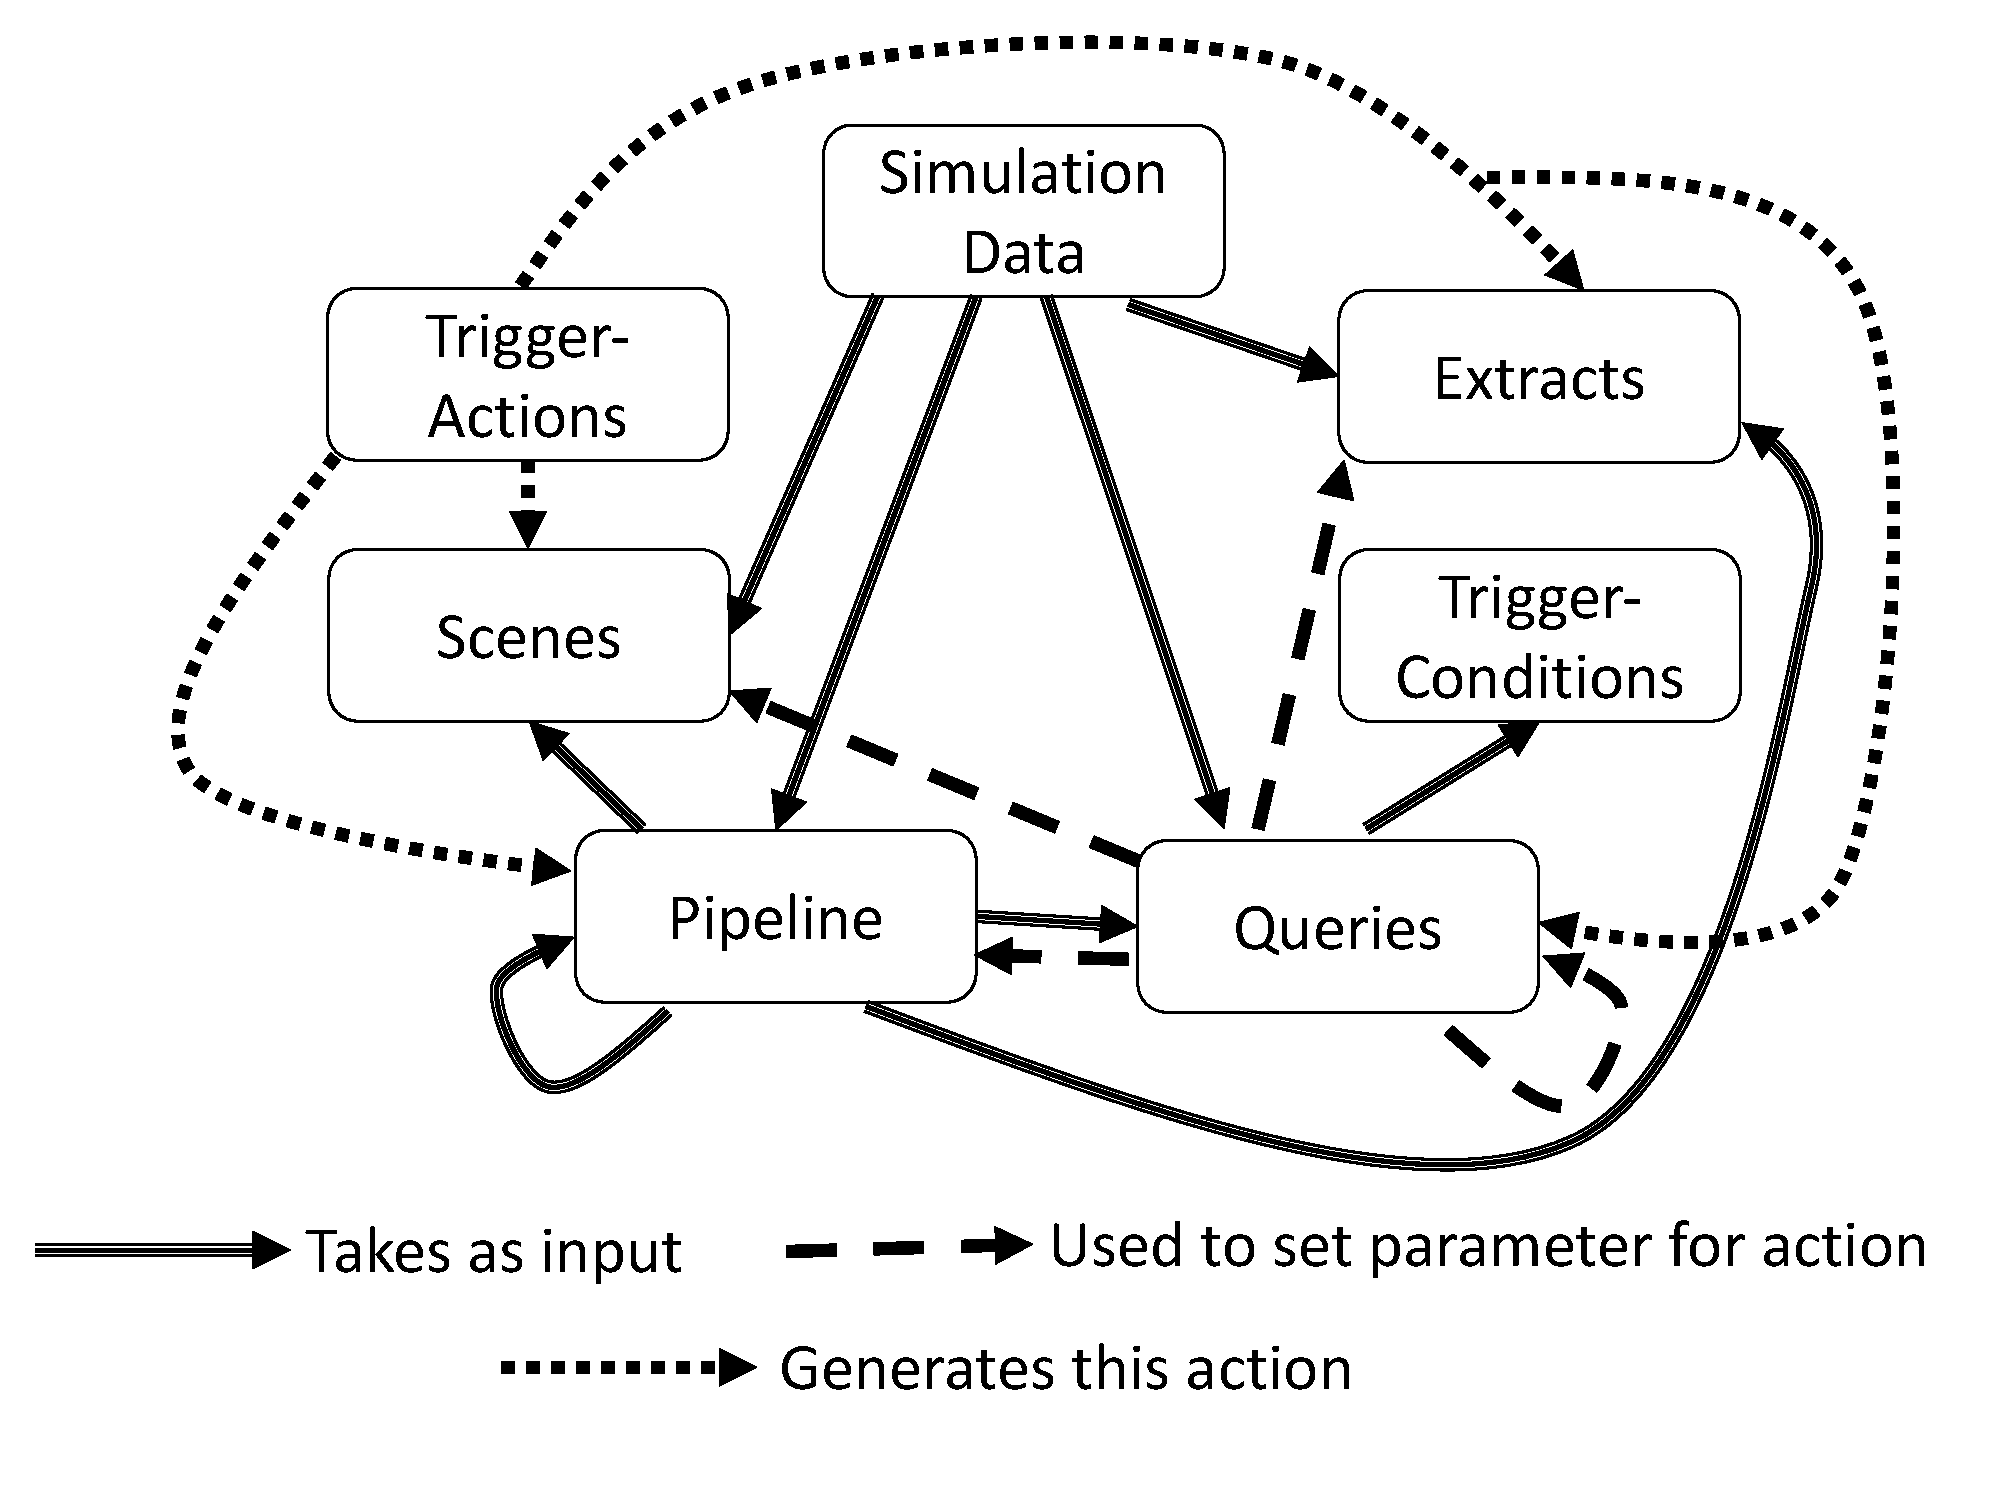
\includegraphics[width=0.75\textwidth]{images/ascent_interactions}
\caption{\label{fig:interactions} Interactions between Ascent actions.}
\end{figure}

Fig.~\ref{fig:interactions} shows interactions between Ascent's actions.
%
It shows three types of interactions via arrow glyphs:
%
\begin{itemize}
\item Takes as input: the action at the tail of the arrow may serve as input for the action at the head of the arrow.
\item Used to set parameter for action: the action at the tail of the arrow may set parameter values for the action at the head of the arrow.
\item Generates this action: the action at the tail of the arrow may generate actions of the type at the head of the arrow.
\end{itemize}

Two of these interaction types are simply described.  
%
First, queries are the only action that can set parameters for other actions, and it does so for
pipelines, scenes, and extracts, as well as for other queries.
%
Second, trigger-actions are the only action that can spawn new actions, and the types it spawns are
pipelines, scenes, extracts, and queries.
%

The last interaction type is on inputs.
%
Simulation data is input to pipelines, scenes, extracts, and queries.
%
Pipelines are input to the same types of actions, meaning that pipelines can serve as input
to other pipelines.
%
Further, in these cases, there can be multiple inputs, e.g., one query can have multiple
pipelines as input.
%
The last input involves queries and trigger-conditions. 
%
In this case, the queries would have their own inputs (i.e., simulation data or pipelines), 
but the trigger-condition would be firing or not based on the result of the query ---
the simulation data or pipeline is one step removed.

Finally, Fig.~\ref{fig:interactions} shows simulation data as only being at the tails of arrows,
and never the heads, i.e., nothing is ever sent to the simulation.
%
In reality, Ascent does have pathing to send data back to the simulation.
%
This is most useful for queries, but also applies to the other actions.
%
For example, it is possible to have a scene return an image (instead of writing it to disk)
and then pass that image back to the simulation (as bytes).


